%----------------------------------------------------------------------------
\section{Javaslat a kockázatok kiszűrésére}
\label{sec:6}
%----------------------------------------------------------------------------

% TODO
% rövid szöveg ide

\subsection{Adversarial módszerek}

A korábban vizsgált megközelítéssel sajnos nem sikerült jó eredményeket elérni. A modell robusztusságából adódóan néhány jellemző kivételével nem romlik a modell pontossága, és a hálózat effektus feltételezés sem bizonyult helyesnek. Következő próbálkozás az adversarial attack módszerek irányába indult. Adversarial examplenek nevezzük azt a mintát, amelyet, ha kis mértékben módosítunk képes becsapni egy adott machine learning modellt. Ezt a gyakorlatban egy kis mértékű pontosan kiszámított zaj hozzáadását jelenti, miközben a modell hibáját maximalizálja. 

Annak érdekében, hogy belássuk, működhetnek az ilyen módszerek azt tűztem ki célul, hogy mutassam be néhány félig manuálisan készített példán keresztül, hogy az arclenyomatok kis mértékű módosításával be lehet csapni a random forest classifier modellünket. Ehhez készítettem egy újabb algoritmust, amelyet előbb Iris dataseten teszteltem a könnyebb értelmezhetőség érdekében, majd miután működött áttértem az arclenyomat vektorok használatára.

Az algoritmus mögöttes ötlete abból ered, hogy ha megvizsgáljuk az egyes döntési fákat, találhatunk olyan elágazásokat (feltételeket) ahol egy adott arclenyomat vektor jellemzőinek értéke a döntési küszöbértékhez meglehetősen közeli értéket vesz fel. Az ilyen esetekben ezeknek a jellemzőknek kis módosításával el lehet érni azt, hogy a döntési fa feltétele átbillenjen, és másik útvonalon halad a következő elágazásig. Ez a módosítás önmagában még nem garantálja azt, hogy a döntési fa kimenete megváltozik, mivel előfordulhat, hogy a kitérítés után egy másik levélre jut, ami ugyanazt az eredményt adja, mint az eredeti kimenet. Ezt szemlélteti a következő példa.

\begin{figure}[ht]
	\centering
	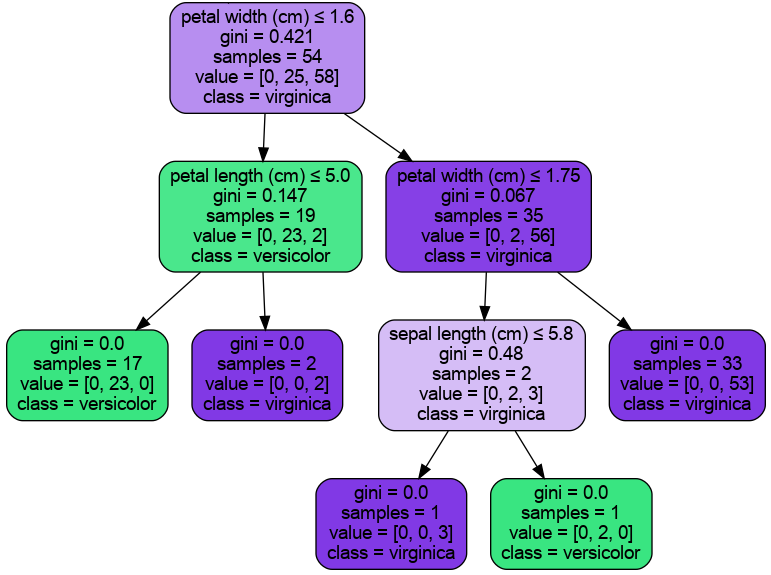
\includegraphics[width=0.9\columnwidth]{figures/adverse_tree_graph.png}
	\caption{Döntési fa részlete, ami az Iris datasetre lett betanítva.}
	\label{fig:iris_tree}
\end{figure}

Tegyük fel, hogy az általunk vizsgált mintában a petal width jellemző értéke 1,55 cm, petal length értéke 4,5 cm. Ezt a mintát a \ref{fig:iris_tree}. ábrán látható döntési fa alap esetben ``versicolor'' kategóriába sorolná. A döntési fa a legfelső elágazásnál petal width $\le$ 1.6 cm feltétel szerepel. Belátható, hogy a bemeneti érték kis módosításával (1.55 + 0.05) átbillenthető a feltétel teljesülése, és az eredeti bal ág helyett jobb ág irányába halad tovább a döntéshozatal, ezzel potenciálisan téves predikcióra vezethető a fa. Azt is láthatjuk ebben a példában, hogy ha a mintánkban a sepal length jellemző értéke nagyobb mint 5,8 cm, akkor újból ``versicolor'' levélre jutunk, tehát előfordulhat, hogy hiába tévesztettük meg a döntési fát egy ponton, a fa predikciója továbbra is változatlan marad.

A véletlen erdő sok döntési fát tartalmaz, amelyek mind képeznek egy-egy szavazatot az egyik kimenetre, ezért egyetlen fa becsapása legtöbb esetben nem elegendő a teljes véletlen erdő kimenetének módosítására, így a bemeneti arclenyomat vektor olyan módosítása szükséges, ami egyidejűleg több döntési fa predikcióját is képes eltéríteni.

\subsubsection*{Adversarial módszer fejlesztése Iris adathalmazon}

Az Iris dataseten betanított random forest classifieren a korábbihoz hasonlóan egy rekurzív függvényt használtam, ami végighalad az erdőben található egyes döntési fákon, és az elágazásoknál vizsgálja az adott feltételhez tartozó jellemző bemeneti értékét, és küszöbértékét. Az algoritmus első verziója egy adott bemenetre keresi azokat a küszöbértékeket, amelyek a bemenettől maximum 10\%-kal térnek el. Ezeknél a feltételeknél van lehetőségünk kis módosítással megtéveszteni a fát. Az ilyen eseteknél a program kiírja melyik fáknál, és melyik jellemző értéknél van megfelelően kis eltérés a küszöbértékhez képest.

\begin{lstlisting}[caption={A döntési azon elágazási pontjai, amelyek kis jellezőmódosítással átbillenthetőek.}]
Tree: 0 out: 1  feature: PL  4.9 <= 4.85, diff: -0.05
Tree: 1 out: 1  feature: PL  4.9 <= 4.95, diff: 0.05
Tree: 2 out: 1  feature: PW  1.5 <= 1.55, diff: 0.05
Tree: 2 out: 1  feature: PL  4.9 <=  5.0, diff:  0.1
Tree: 3 out: 1  feature: PL  4.9 <= 4.95, diff: 0.05
Tree: 4 out: 1  feature: PL  4.9 <= 4.95, diff: 0.05
Tree: 5 out: 1  feature: PL  4.9 <= 4.95, diff: 0.05
(*@\raisebox{-1pt}[0pt][0pt]{$\quad\vdots$}@*)
Tree: 99 out: 1  feature: PW  1.5 <= 1.55, diff: 0.05
\end{lstlisting}

Az eredményeket megpróbáltam valamilyen módon összesíteni, de voltak esetek mikor a küszöb érték alatt volt a jellemző értéke kicsivel, volt mikor fölötte. Az könnyen látható volt, hogy a petal length feltétel szerepelt a 100 fából leggyakrabban, így annak a módosításával próbálkoztam.

A módszer szemléltetésére kerestem egy mintát, ahol a véletlen erdő fái egyértelműen döntöttek az egyik osztály mellett, és a bemenet kis módosításával próbáltam elérni, hogy minél több fa téves predikcióra jusson. Az alábbi mintánál eredetileg a 96 szavazott a ``versicolor'' osztályra, majd egyetlen jellemző viszonylag kis módosítással (petal width 4,9-ről 5.05-re lett növelve) sikerült elérni, hogy a fák többsége ``virginica'' osztályra szavazzon.

\begin{lstlisting}[caption={A véletlen erdő kimenetének manipulációja.}]
Eredeti értékek:
[6.9 3.1 4.9 1.5]
Módosított értékek:
[6.9  3.1  5.05 1.5 ]
Módosítás mértéke:
0.88%

Fa szavazatok:
módosítás előtt [ 0. 96.  4.]
módosítás után  [ 0. 40. 60.]
\end{lstlisting}

\subsubsection*{Adversarial módszer arclenyomat vektorokon}

Az Iris datasetes példán elért eredmények után az algoritmus fejlesztését az arclenyomat vektorokról készült adathalmazon folytattam. Az algoritmus működése során továbbra is végighalad a döntési fán és a bemenet értékeitől függően lép egyik elágazásról a következőre. Ennél a verziónál is detektáltam az olyan elágazásokat, ahol a bemeneti érték egy előre definiált tartományon belül tér el a küszöbértéktől. Minden alkalommal, mikor detektál az algoritmus egy ilyen elágazást, az elágazás mindkét ágán folytatja a fa feltérképezését egészen addig, amíg levél csomóponthoz nem jut. A levélhez eljutva megnézi, hogy az adott levélhez tartozó kimeneti osztály megegyezik-e a mintához tartozó címkével, vagy sem.

Itt az az elgondolás, hogy minden esetben mikor könnyen átbillenthető csomóponthoz jutunk, eldönthetjük, hogy melyik úton érdemes tovább haladni. Az egyes lehetséges utakat feltérképezve ki tudjuk választani azt az utat, ami téves predikcióhoz vezet, illetve, ha több ilyen út van akkor ki tudjuk választani azt, amelyikhez a legkisebb beavatkozás szükséges. 

Az algoritmus végig megy a véletlen erdő összes döntési fáin, kivéve azokat, amelyek alapból is téves predikciót adnak, mivel ezeken nem kell módosítanunk.

\begin{lstlisting}[caption={Algoritmus futtatása egy adott arclenyomat vektorra.}, label=lst:tree_diffs]
Tree: 4, output: 3
		f10  diff: -0.0267
Tree: 4, output: 2
		f88  diff: -0.04035
Tree: 9, output: 3
		f77  diff: -0.02279
Tree: 11, output: 3
		f93  diff: 0.002902
		f57  diff: -0.008323
		f82  diff: -0.007353
Tree: 11, output: 3
		f93  diff: 0.002902
		f57  diff: -0.008323
		f91  diff: 0.02286
(*@\raisebox{-1pt}[0pt][0pt]{$\quad\vdots$}@*)
Tree: 48, output: 1
		f93  diff: 0.002753
\end{lstlisting}

Az algoritmus lefuttatható egy adott arclenyomat vektorra. Lefuttatás során a \ref{lst:tree_diffs}. kódrészlethez hasonló információt kapunk. Eredményül egy listát kapunk, ami felsorolja azokat a fákat a random forest classifier-en belül, amelyek kis (10\% alatti) input módosítással megtéveszthetőek. Fel van tüntetve a fa sorszáma, illetve a fa megtévesztés utáni predikciója (ennél a példánál helyes predikció 0 lenne.) Egy fához fel vannak sorolva azok a jellemzők amelyeket módosítani kell a fals predikció eléréséhez, ahol a ‘diff’ érték mutatja a szükséges módosítás mértékét. Ha több jellemző van felsorolva, például Tree 11-nél akkor azok a módosítások ÉS kapcsolatban állnak egymással.

Megfigyelhetjük ezen a példán, hogy egy fához több téves predikció is tartozhat, attól függően, hogy melyik jellemzők értékét változtatjuk. Például a Tree 4 esetén elérhetünk 3-mas vagy 2-es predikciót is. Az is előfordulhat, hogy egy döntési fán belül több útvonal vezet egy téves predikcióhoz, például Tree 11 esetén három féle képen kaphatunk 3-mas predikciót. Ilyenkor a kisebb módosítást igénylő út a preferált. 

Jelenleg az algoritmus félig automatikus működésű. A lefuttatás során nem fog módosítani az eredeti mintán, azt manuálisan kell elvégezni. Ez az egyik terület, ahol tovább szeretném fejleszteni ezt a megoldást, hogy képes legyen kiszámolni az optimális átalakítást, ahol a legkisebb zaj hozzáadásával megtéveszthető a véletlen erdő becslése. Jelenleg kézzel lehet összeválogatni az egyes jellemzők módosításait, és az alapján összerakni egy zaj vektort. A feladat nehézségét az adja, hogy lehetnek ellentmondásos feltételek (egyik fa növelni szeretné a jellemző értékét, másik pedig csökkenteni), illetve az is előfordulhat, hogy egy jellemző módosítás hatására az egyik fánál korábbi rossz predikció átvált helyesre. Az jellemző módosítások optimális kombinációjának megtalálása nem egyszerű feladat.

\begin{lstlisting}[language=python, caption={Korábbi elemzés alapján manuálisan elvégzett jellemző módosítások.}, label=lst:tree]
# feature modositasok
x_ = x.copy()

x_[:,10] += -0.0268  # Tree 4, Tree 17
x_[:,77] += -0.0228  # Tree 9
x_[:,43] += -0.02737  # Tree 13, 29, 31
x_[:,8] += 0.02539  # Tree 24
x_[:,88] += -0.0314  # Tree 35
x_[:,105] += -0.02175  # Tree 37
x_[:,44] += 0.02302  # Tree 41

print('tree votes:')
print(count_votes(x))
print(count_votes(x_))

# kimenet:
'''
tree votes:
[30. 4. 3. 13.]
[20. 4. 4. 22.]
'''
\end{lstlisting}

A \ref{lst:tree}. kódrészleten láthatjuk, hogyan végezhető el a korábban megállapított jellemzők módosítása. Az eredeti arclenyomat vektor értékeit az ‘x’ változó tárolja. A random forest classifier 50 fából áll, melyek közül 30 fa eredetileg 0 predikciót képez. Egy-egy jellemző módosításnál kommentben megneveztem azokat a fákat, amelyeknek a módosítás hatására átváltanak a helyes (0) predikcióról egy másik értékre. Összesen 10 fa megtévesztésével elérhettük azt, hogy a teljes erdő téves predikciót produkál a módosított mintára. 

Fontos még megjegyezni, hogy összességében elég kis módosítással sikerült elérni ezt az eredményt. Az arclenyomat vektor 128 jellemző közül elegendő volt 7-et kiválasztani, és azokat is maximum 10\%-ban módosítani. A feltételezésem az, hogy ez a módosítás elegendően specifikus és kis méretű, hogy ezzel még megőrizhető egy arclenyomat vektorok alapján betanított identifikációs modell pontossága, de ezt még nem teszteltem le.

\subsubsection*{Összefoglalás}

Ebben a dokumentumban összefoglaltam a félév alatt Diplomatervezés 1 tantárgy alatt elvégzett munkám eredményeit. A félév első felét hálózat effektus hipotézis vizsgálatával töltöttem, ami végül nem vezetett eredményre. Bemutattam a hipotézis mögött rejtő gondolatmenetet és a kísérleteket.

Később az adversarial attack jellegű algoritmus fejlesztésével foglalkoztam. Bemutattam a döntési fák vizsgálatának módszerét és implementálását. Részleteztem az algoritmus fejlesztésének menetét, az egyszerűbb feladatok megoldását, majd az arclenyomat vektorokon elért eredményeket.Jelenleg az algoritmus félig automatikus működésű, azaz a döntési fák elemzése után kézzel kell összeállítani az arclenyomat vektorok módosítását. Az egyik főbb továbbfejlesztési irány az lenne, hogy az algoritmus képes legyen közel optimális zaj generálására, amellyel a véletlen erdő predikciója becsapható. 

E mellett meg kell még vizsgálnom, hogy az arclenyomat vektor módosítása során mennyire romlik az arclenyomat felhasználhatósága egyéb célokra, például identifikációra? Sikerül-e reprodukálni az eredményeket más adathalmazokon betanított modelleken? További irány lehet más területeken sikeresen alkalmazott adversarial attack módszerek kipróbálása véletlen erdő modellre, és az eredmények összevetése.

\subsection{Titkosítási módszerek}

4-5 oldal
\begin{itemize}
	\item titkosítási módszerek előnye
	\item lsh
	\item random projekció
\end{itemize}
% javaslat: titkosítás, lsh, random projekció %(source: MNB arcfelismerés)